\section{Results and evaluation}
\label{sec:Auswertung}
Calculations with the resulting data are done digitally with the programming language \enquote{Python}.
Multiple packages are used, such as \enquote{Matplotlib}~\cite{matplotlib} for creating graphics, \enquote{SciPy}~\cite{scipy} for physics constants and curve-fitting and \enquote{Numpy}~\cite{numpy} for data management and math support.
The uncertainty management as stated in \autoref{sec:fehlerrechnung} is done with the \enquote{Uncertainties}-package~\cite{uncertainties}.
\begin{figure}
  \begin{subfigure}{0.48\textwidth}
    \centering
    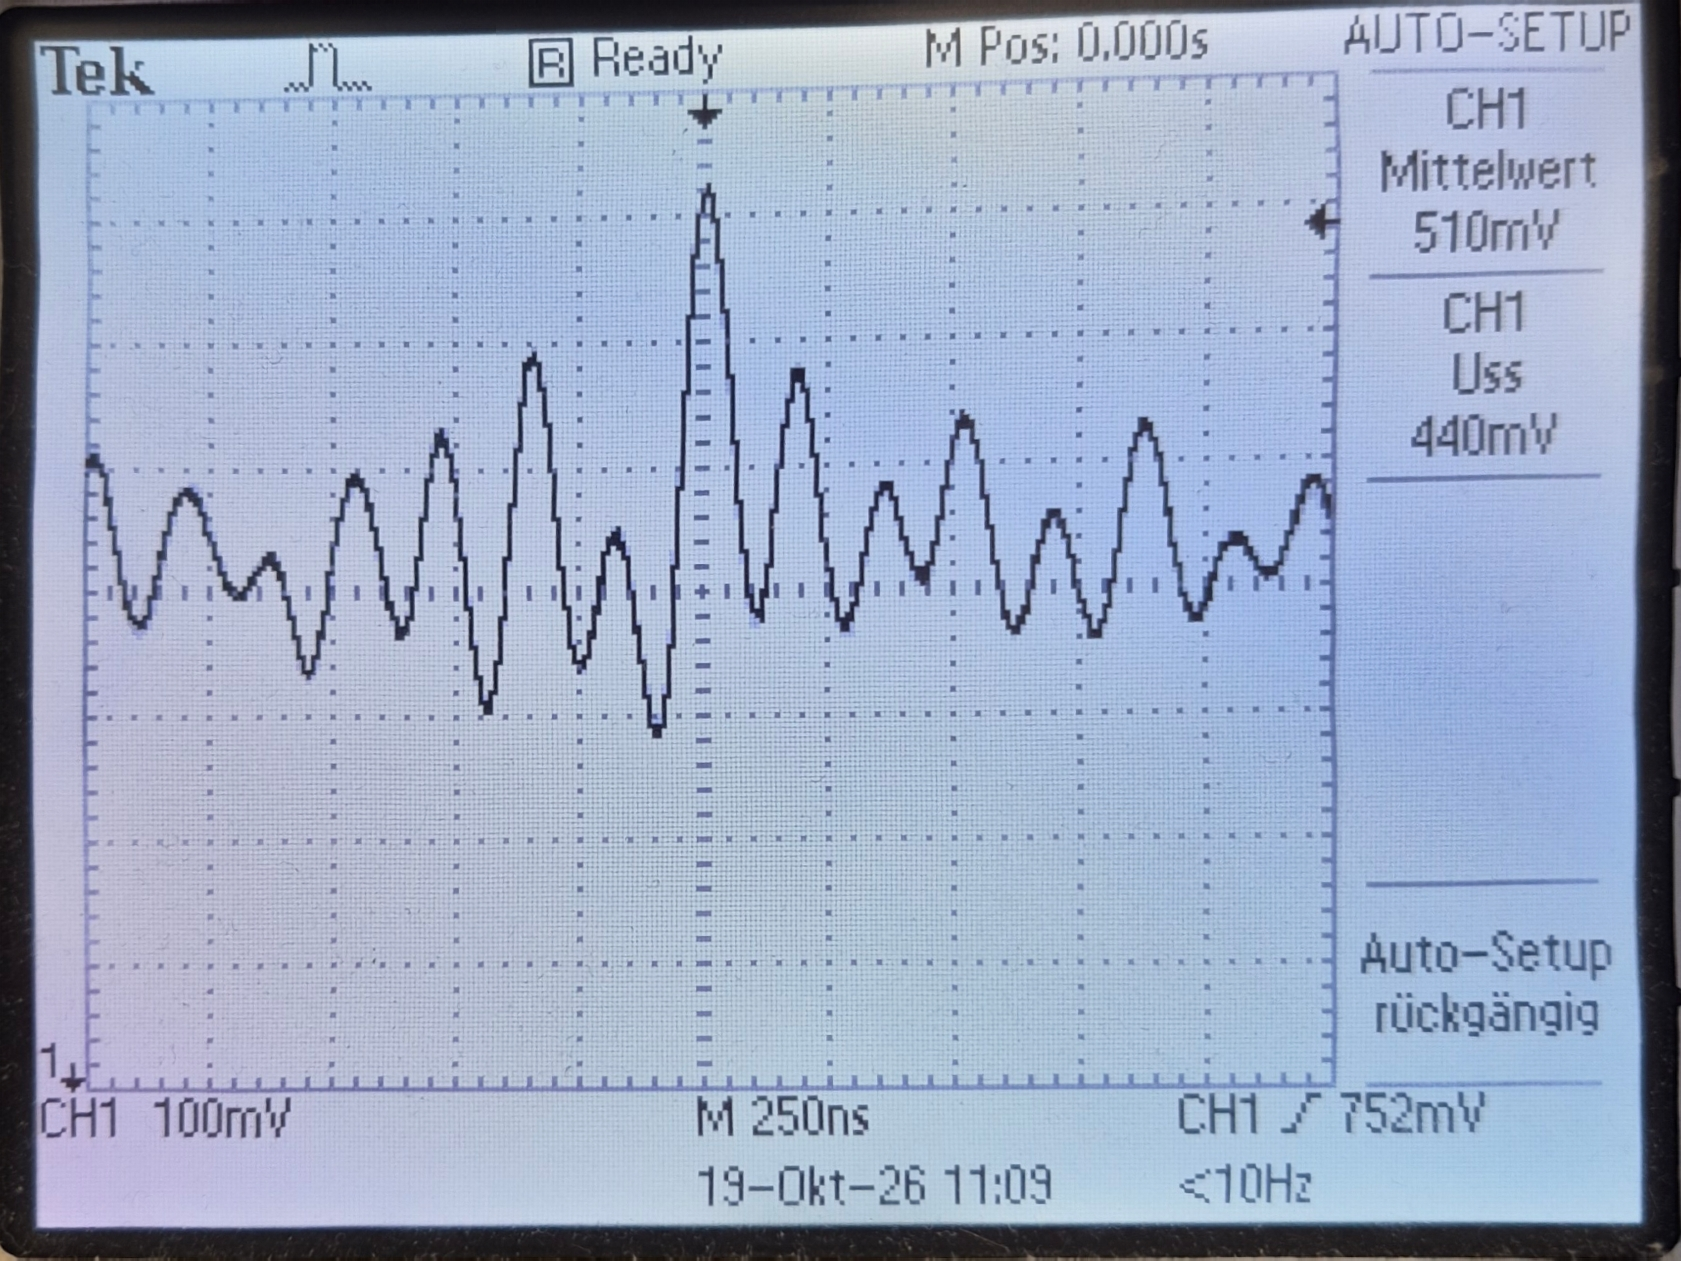
\includegraphics[height=5cm]{content/images/pre-amplified.jpg}
    \caption{Not amplified signal.}
    \label{subfig:pre}
  \end{subfigure}
  \hfill
  \begin{subfigure}{0.48\textwidth}
    \centering
    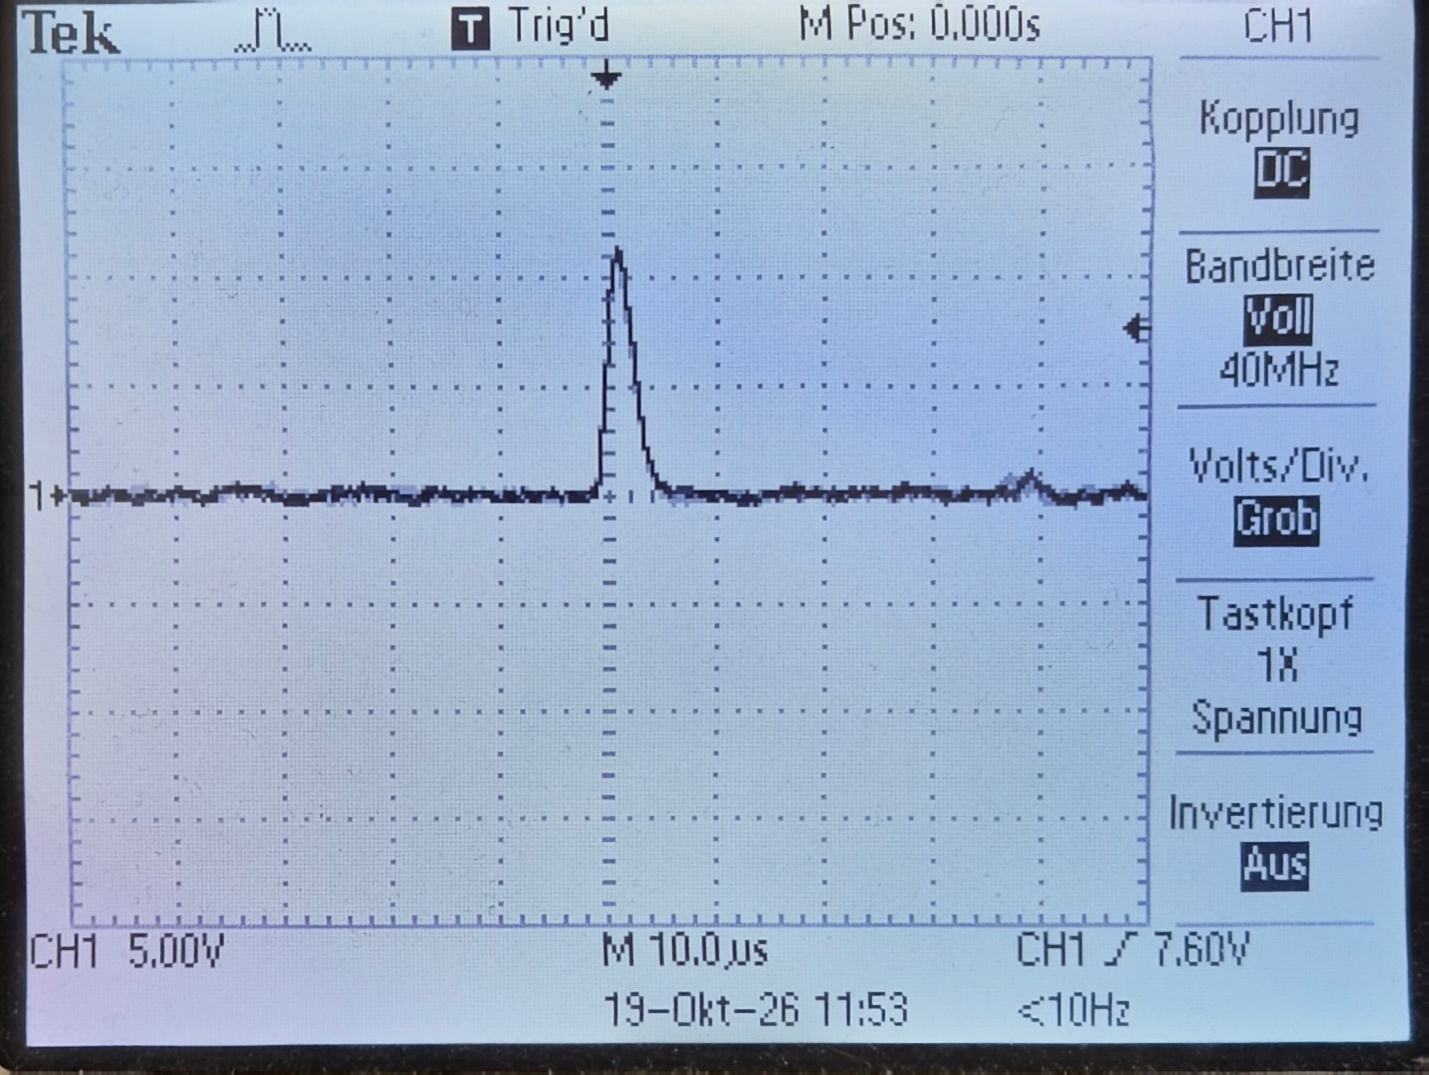
\includegraphics[height=5cm]{content/images/amplified.jpg}
    \caption{Amplified signal.}
    \label{subfig:after}
  \end{subfigure}
  \caption{Detector pulses before and after amplification, shown on a digital oscilloscope.}
  \label{fig:pulses}
\end{figure}
\FloatBarrier
